	\documentclass[10pt]{article}
\usepackage{graphicx}
\usepackage{float}
\usepackage{amsmath}
\usepackage[margin=0.7in]{geometry}
\usepackage{caption}
\usepackage{subcaption}
\usepackage{multicol}

\restylefloat{figure}
	\title{IT3708 - Exercise 3}
\author{
        Eirik Hammerstad \& Nicklas Utgaard
}
				
\date{\today}
\begin{document}
\maketitle
%\pagebreak
%\tableofcontents
%\pagebreak
\section{Overview}
	\subsection{System}
		The system used to solve this exercise consists of four maven projects\footnote{Maven - http://maven.apache.org/}, 
		\begin{table}[H]
			\begin{tabular}{ll}
				\textbf{GA} & Genetic algoritm framework\\
				\textbf{ANN} & Artificial neural network framework\\
				\textbf{TrackerGame} & TrackerGame implementation and APIs\\
				\textbf{CTRNNBundle} & The exercise specific classes, and bundling of all dependencies.
			\end{tabular}
			\caption{The overall structure for this exercise can be seen in figure~\ref{fig:struct}.}
			\label{tabel:project}
		\end{table}
The architecture for GA has been covered in previous deliveries in this course, and will therefor not be covered here. We will however give a brief introduction to the new projects within this exercise. 
		
	\textbf{ANN}(Figure~\ref{fig:annstruct}) gives the basis building blocks for building artificial neural networks, it is large based around the same structure one would see in graph problems\footnote{Graph theory - http://en.wikipedia.org/wiki/Graph\_theory}, but with the addition of \textit{NeuralLayer}. In comparison to normal graphs the nodes has been replaces by neurons and the edges replace by synapses. Though the \textit{NeualLayer} abstraction is not necessary it provides and easy way of structuring the network. To bring it all together and keep track of the network we have \textit{StructuredANN}.

		\textbf{TrackerGame}(Figure~\ref{fig:trackergamestruct}) is the implementation of the game described in the exercise description. It consist only of two entities, \textit{World} and \textit{TrackController}. \textit{World} is the govering entity, in charge of updating the models, and asking the \textit{TrackController} for its next move. 

		\textbf{CTRNNBundle} is the project that combines all the project into one runnable project and makes the exercise specifics implementations needed for the evolutionary algorithm (genotype, phenotype, population creator, fitnesshandler, plotting ect.). The most interesting classes in this project is \textit{ANNBuilder} and \textit{ANNTrackerController}. \textit{ANNBuilder} is the class in charge of converting the parameter array evolved into a working artificial neural network. \textit{ANNTrackerController} is a supporting class for the fitnesshandler, and preforms the simulation of the game with a neural network as the controller in order to determind the fitness of the  neural network parameters. The genotype and phenotype implementations is discussed in the next section. 
		
	\begin{figure}
		\centering
		\begin{subfigure}{.3\textwidth}
			\centering
			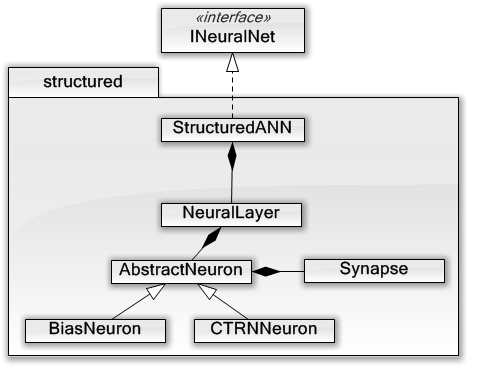
\includegraphics[width=\linewidth]{./../images/ANN.png}
			\caption{ANN structure}
			\label{fig:annstruct}
		\end{subfigure}
		\begin{subfigure}{.3\textwidth}
			\centering
			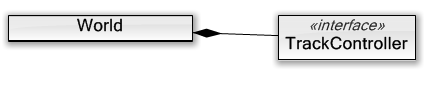
\includegraphics[width=\linewidth]{./../images/TrackerGame.png}
			\caption{TrackerGame structure}
			\label{fig:trackergamestruct}
		\end{subfigure}
		\begin{subfigure}{.3\textwidth}
			\centering
			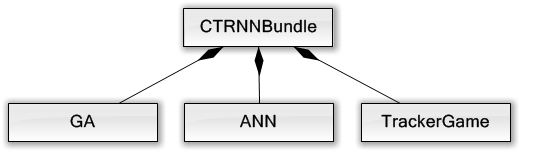
\includegraphics[width=\linewidth]{./../images/Structure.png}
			\caption{Project structure}
			\label{fig:struct}
		\end{subfigure}
	\end{figure}

	\subsection{Genotype}
		We chose a binary representation of our genotype with 8 bit accuracy. This representation is extremely similar to the one used in the previous exercise. The only big difference is the shear number of parameters (5 in previous exercise. 34 in this one, 26 weights, 4 gains, 4, time constants), which results in a much larger bitvector (272 bits). The transformation from binary to real values is however the same. 
	\begin{table}[H]
		\parbox{.45\linewidth}{
			\centering
			\begin{tabular}{ll}
				0..4 & gains for hidden then output\\
        4..8 & time constants for hidden then output\\
        8..18 & weights originating in inputlayer\\
				18..26 & weights originating in hiddenLayer\\
        26..30 & weights originating in outputlayer\\
				30..34 & weights originating in baislayer
			\end{tabular}
			\caption{Structure of bitvector}
		}
		\hfill
		\parbox{.45\linewidth}{
			\centering
			\begin{align}
				param &\in \{p_1, p_2, \dots, p_n\}\nonumber\\
				acc &= 8\nonumber\\
				bitvector &= 00001101\dots11100110\nonumber\\
				bitvector_{param} &= subvector(bitvector, param)\nonumber\\
				coef_{param} &= (bitvector_{param})_{10}\nonumber\\
				step_{param} &= (max_{param}-min_{param})/2^{acc}\nonumber\\
				param &= min_{param}+(coef_{param}*step_{param})\nonumber
			\end{align}
			\caption{Bitvector conversion}
		}
	\end{table}
	
	\subsection{Parameters}
		\begin{table}[H]
			\parbox{.45\linewidth}{
				\centering
				\begin{tabular}{ll}
					Adult selection protocol & Generational mixing\\
					Parent selection mechanism & Sigma scaling\\
					Population size & 100\\
					Number of generations & 1000\\
					Crossover rate & 0.9\\
					Mutation rate & 0.1
				\end{tabular}
				\caption{Evolution algorithm parameters}
			}
			\hfill
			\parbox{.45\linewidth}{
				\centering
				\begin{tabular}{ll}
					Tracker size & 5\\
					Object size & [1, 6]\\
					Arena size & 30 x 15\\
					Tracker speed & [-4, 4]\\
					Capture ratio & 1.0\\
					Avoidance ratio & 0.0
				\end{tabular}
				\caption{Tracker scenario parameters}
			}
		\end{table}
\section{Verification}
	We used a score based fitness function related to the number of shadows registered and the size of the object. In addition to fitness gained by catching or avoiding object, we rewarded fitness based on the speed. This was done to make an incentive to utilize speed and therefore increase the probability of reaching an object in time. The reward for catching or avoiding an object was calculated each time an object reached the bottom of the arena, while the speed reward was accumulated at each time step based on the reaction of the tracker. The basic formula for out fitness is as show below, with the different rewards varying depending on our goal.
	\begin{align}
		fitness &= \alpha catch\_reward+\beta avoid\_reward+\theta speed\_reward\nonumber\\
		ratio(shadows, size) &= \frac{shadows}{size}\nonumber
	\end{align}
In order to gauge the outcome when an object reached the bottom we use the ratio shown above, where $shadows$ is the number of shadows on the tracker, and $size$ is the size of the falling object.

In order to find the best possible parameters for evolving a solution to this project we used a parallel exhaustive search in parameter space, with a fixed population size of 100, 200 generations. The top 20 cases were tested 20 induvidual times to find the parameters generating the 'on average' best solution. 
	\subsection{Catch all}
		\subsubsection{Fitness function}\label{sec:fitness1}
			\begin{align}
				catch\_reward(shadows, size) &= \left\{ 
				\begin{array}{l l}
					2 &\text{if $ratio=1$ and $object\_size <= 5$} \\
					2 &\text{if $ratio>0.8$ and $object\_size = 6$}\\
					0 &\text{else}
       \end{array} \right.\nonumber\\
				avoid\_reward(shadows, size) &= 0\nonumber\\
				speed\_reward(speed) &= \left\{ 
				\begin{array}{l l}
					0.000 &\text{if $|speed| < 2$} \\
					0.003 &\text{if $|speed| = 2$} \\
					0.006 &\text{if $|speed| = 3$} \\
					0.009 &\text{if $|speed| = 4$} \\
       \end{array} \right.\nonumber\\
			 \alpha =\beta =\theta &= 1\nonumber
			\end{align}
		\subsubsection{Parameters}
			From our tests, exhaustive search with 20 cases of the 20 best found, we found that while using sigma scaling selecton mechanism a high mutation rate ($0.3-0.4$) yielded the best result. When sorting the average of each case we saw that the sigma scaling to a large degree dominated over a tournament based selection mechanism with a 5\% drop in fitness between the worst average using sigma scaling and best average of using a tournament best selection mechansim.
		\subsubsection{Results}
			The best average result we got scored 67.22 points out of a total of 85.4 (79\% of total). 
			The parameters used to obtain this result can be seen in table~\ref{tab:resultAll}. 
			\begin{table}[h]
				\parbox{.45\linewidth}{
					\centering
					\begin{tabular}{ll}
						Parameter & Value\\\hline
						Selection Protocol & Generational mixing\\
						Selection Mechanism & Sigma scaling\\
						Crossover rate & 0.7\\
						Mutation rate & 0.4\\
						Population size & 100\\
						Number of generations & 200
					\end{tabular}
					\caption{Parameters used to obtain best average case}
					\label{tab:resultAll}
				}
				\hfill
				\parbox{.45\linewidth}{
					\centering
					\begin{tabular}{ll}
						Number of runs & 20 \\
						Best run & 80.816\\
						Worst run & 50.5\\
						\hline
						Average fitness & 67.22\\
						Standard deviation & 8.7\\
					\end{tabular}
					\caption{Results for best case}
					\label{tab:resultAll}
				}
			\end{table}
	\subsection{Catch and avoid}
		We used the same approch as earlier to determind the best average for a given set of parameters to the evolutionary algorithm. The 20 best of an exhaustive search was picked out and tested by running them 20 more times. 
		\subsubsection{Fitness function}
			The fitness function we used to evolve both catching and avoiding is in the great scheme of things similar to the one described in section~\ref{sec:fitness1}. The modifications can be seen below.
			\begin{align}
				catch\_reward(shadows, size) &= \left\{ 
				\begin{array}{l l}
					2 &\text{if $ratio=1$ and $object\_size < 5$} \\
					0 &\text{else}
       \end{array} \right.\nonumber\\
				avoid\_reward(shadows, size) &= \left\{ 
				\begin{array}{l l}
					2 &\text{if $ratio=0$ and $object\_size >= 5$} \\
					0 &\text{else}
       \end{array} \right.\nonumber\\
			\end{align}
		\subsubsection{Behaviour}
				Our agent moves in the same direction at all times with a speed of 2 when it does not see any shadows. Upon receiving input from on or more of its shadow sensors it speeds up to 3 in order to get under the object as fast as possible. When it is under the object it is able to determind the size of the object, if the object should be catched it usually stops and waits for the object, in the case where it sees a big object it continues to speed up to 4 and gets away from the object. There are some issues with this agent, in some cases it speeds up to much in order to avoid an object and ends up going a full circle before the object land on top of the tracker. Another problem is with spawning of new objects that partially cover the shadowssensor, in this case it does not recognize that it is a new object and continues to wait for it to land. But in most cases it is very successful in its behaviour.
		\subsubsection{Result}
			The best average result we got scored 51.11 points out of a total of 85.4 (60\% of total). 
			The parameters used to obtain this result can be seen in table~\ref{tab:resultAvoid}. 
			
			In general we found that a fitness above 50 will behave logically in one or another way related to the task at hand. From our test trails we had 156 different networks that scored over 50 in fitness, and 26 that had over 60. This is based on a total of 1012 different runs. 
			\begin{table}[h]
				\parbox{.45\linewidth}{
					\centering
					\begin{tabular}{ll}
						Parameter & Value\\\hline
						Selection Protocol & Generational mixing\\
						Selection Mechanism & Sigma scaling\\
						Crossover rate & 0.9\\
						Mutation rate & 0.5\\
						Population size & 100\\
						Number of generations & 200
					\end{tabular}
					\caption{Parameters used to obtain best average case}
					\label{tab:resultAvoid}
				}
				\hfill
				\parbox{.45\linewidth}{
					\centering
					\begin{tabular}{ll}
						Number of runs & 20 \\
						Best run & 64.66\\
						Worst run & 41.00\\
						\hline
						Average fitness & 51.11\\
						Standard deviation & 7.83\\
					\end{tabular}
					\caption{Results for best case}
					\label{tab:resultAvoid}
				}
			\end{table}
			\begin{figure}%
				\centering
				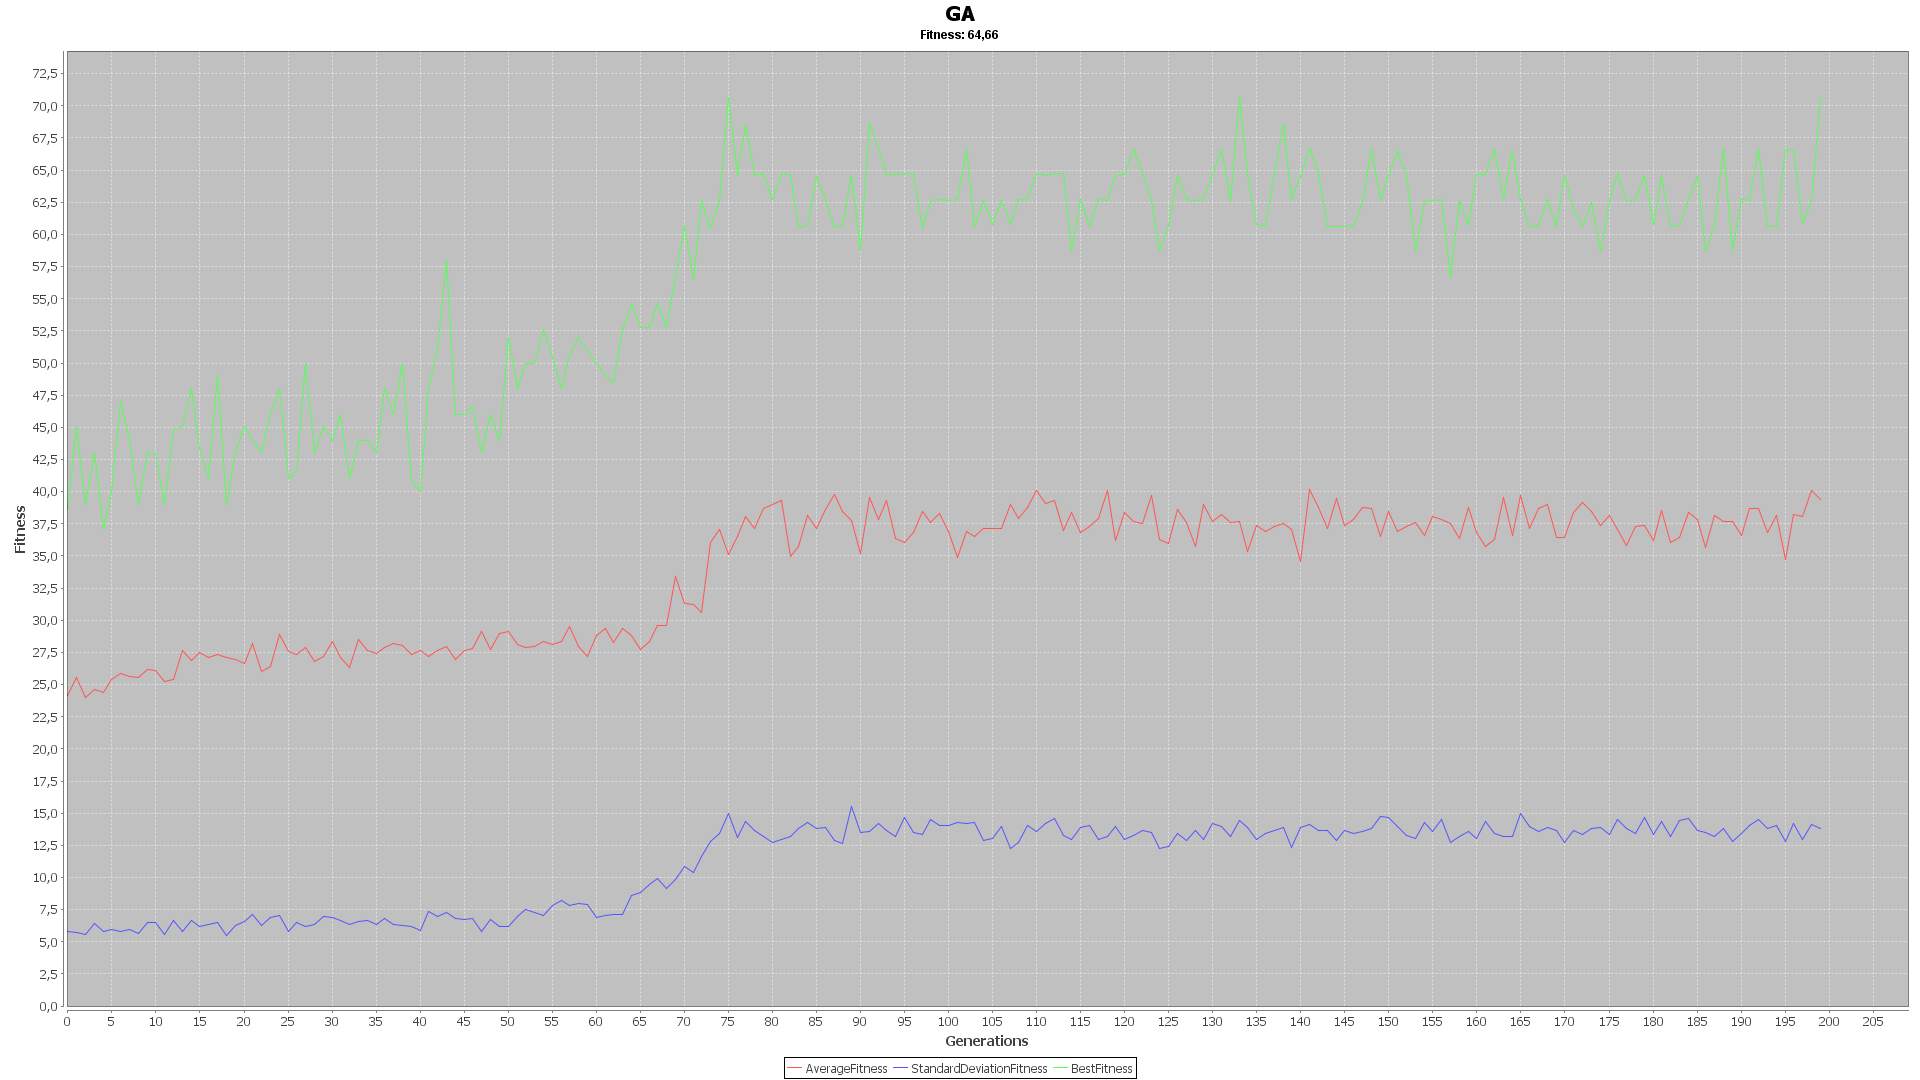
\includegraphics[width=.7\columnwidth]{./../images/fitnessplot.png}%
				\caption{Fitness plot of best run in best average case}%
				\label{fig:best}%
			\end{figure}
\section{Modified tracker scenario}
	\subsection{The change}
		In this task we decisded to change the height and width of the tracker arena. The original size of the arena was 30 wide and 15 high, we changed these to 50 wide and 25 high. No other parameters was changed during this phase of the project. 
	\subsection{Result}
		The changed made resulted in a lower fitness overall. In the original arena we had a best average of 51.11, this was reduced to 45.96 in the big arena(extracted from reruns of top 20). The overall best result from a single run was also greatly reduced, in the original arena we found 68.88 as the best, while in the big arena 63.44 was the best found(extracted from 1012 different run on each arena). 
		
		Though the fitness function was not changed we see a change in both the average best, and single best. In both cases about 5 in fitness was lost. Based on the different "`personalities "` we have seen from our trackers, we believe that there can be several explanations to why it yields a lower fitness overall, with the width of the arena being the greatest influential factor. In many cases we have seen trackers that don't utilize their full speed range, many of them prefers keeping a relative low speed at around 1-2. In some cases this may mean that the tracker never discovers the object before it has allready landed. But due to the ratio between the height and width being the same as in the original scenario, we don't believe this to be the deciding factor. In order to find an explanation to the lowered fitness we tried looking at how the tracker experienced the environment, the main difference we found between the two arenas was the amount of timesteps the tracker would go without seeing an object. This long exposure to the same input combined with the neural network's memory could cause it to skip the smallest object(1s and 2s) since it doesn't manage to deaccelerate to a standstill before it has passed the object. 
		
\section{Modified topology}
	
\section{Modified variable ranges}
\section{In depth}
\section{Appendix}
	
\end{document}